%%
%%############################
\chapter{FSI Tutorial}
\label{tut_fsi:chap}

%%
%%============================
\section{Introduction}

This tutorial will explain how the solving of finite element problems
-- especially fluid structure inteaction examples -- with the LNM
code is done.

In order to keep it as simple as possible, we will mainly focus on
a step by step example here. If you wish to get more detailed explanations,
after each major step there are sections with some more background
information. The idea is that you can follow the example without any
reading any background information in a first attempt and come back
later for more details.

As our example, we will use a very basic scenario here, the so called
driven cavity. Imagine a two dimensional, rectangular chamber, as
sketched in \ref{tut_fsi:1.1}.

%
\begin{figure}[h]
\hfil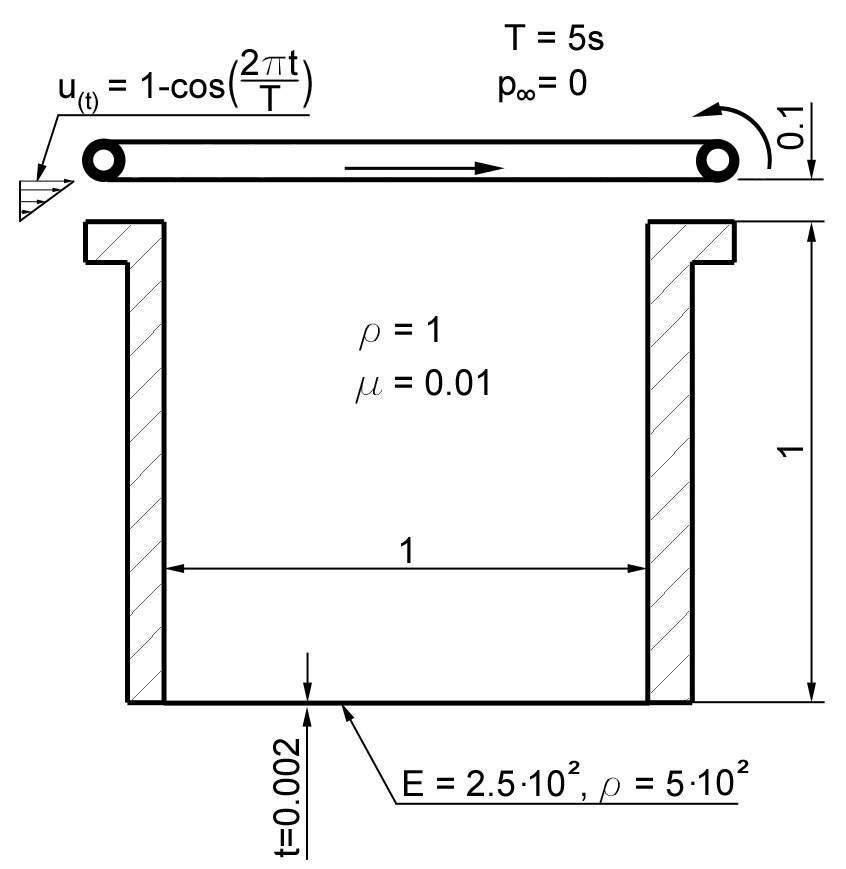
\includegraphics[scale=0.2]{Bilder/Angabeskizze}


\caption{\label{tut_fsi:1.1} The driven cavity example}
\end{figure}


On the top of this chamber, fluid with a certain oscillating velocity
(with triangular distribution) is driven through the chamber. All
of the walls -- except of the bottom -- are assumed to be rigid. Due
to the oscillating motion at the top, the bottom will deform dynamically.

As the FSI preprocessing is quite complex, we will split the example
in three parts:

\begin{enumerate}
\item First we'll study the structure (the bottom) only. We will load it
for simplicity with the stationary fluid weight only.
\item Next we will simulate the fluid in a completely rigid chamber (we
neglect the deformation of the bottom for simplicity).
\item And in the end we will set up the whole example as an FSI simulation.
\end{enumerate}
It is highly recommended to follow this tutorial right from the beginning
step by step, as problems always arise by themselves - trust me, it's
easier that way.


\section{Setup of the LNM-code}

As science at LNM doesn't focus on preprocessing, BACI (the code)
is a solver only.

This means, you have to do the pre- and the postprocessing in a commercial
program (here: GID and Paraview). 

If you need more information on this software than provided here,
you can also refer to a special GID/Paraview tutorial, or - regarding
BACI - the LNM beginners guide.

The preprocess software writes, after a successful input, a \emph{{*}.dat}
file containing all the information of the example (nodes, elements,
boundary conditions,..), which is then given to BACI for solving.
In order to use BACI for your special purposes (here: FSI), you have
to do kind of a setup first. This is done by changing the \emph{defines.dat}
file in the \emph{ccarat/config/} directory. Open it and select the
packages you need by uncommenting the according line. For all we do
here (and also for the third dimension) you will need the following,
so

\begin{itemize}
\item uncomment:

\begin{itemize}
\item Elements: D\_ALE, D\_BRICK1, D\_FLUID2, D\_FLUID3, D\_SHELL8, D\_WALL1;
\item Additional features: BINIO, SOLVE\_DIRICH, SOLVE\_DIRICH2, CCADISCRET;
\item Tools: RESULTTEST, PERF;
\item Fancy stuff: COLOROUTPUT, DSERROR\_DUMP;
\item Possible solver packages: AZTEC\_PACKAGE, UMFPACK, TRILINOS\_PACKAGE;
\item Constants: MAXNOD=9, MAXELE=9, MAXDOFPERNODE=6, MAXGAUSS=9;
\end{itemize}
\item Save the changed \emph{defines} file in the same directory as e.g.
\emph{defines.my.dat}. 
\item Next in the console the call (in the ccarat directory) \emph{./configure
config/muench.fc6.ser config/defines.my} creates the makefile needed
in the following steps. 
\item Use \emph{make clean} before recompiling. 
\item Next simply run \emph{make}.
\end{itemize}
This created everything necessary for BACI to solve your specific
problem.


\section{First structural try}

As already mentioned in the introduction, we will simulate the bottom
of the driven cavity loaded with the stationary fluid weight here.

To start the preprocess, open GID and make yourself familiar with
the very sophisticated desktop. Try to get comfortable with the zoom
and pan tools in the left bar, as they won't be explained any further
in this tutorial (refer to the GID handbook if necessary).


\subsection{General stuff}

\begin{itemize}
\item Activate \emph{Data$\to$Problem type$\to$lnm\_general.}
\end{itemize}
This is necessary in order to make it possible for BACI to read the
output of GID (the \emph{{*}.dat} file). You have to use \emph{lnm\_general}
as basis for everything you want to solve with BACI. You then get
access to menus like \emph{Data-Conditions-SingleLayer} where you
define boundary conditions, elements etc.

\begin{itemize}
\item In \emph{Data$\to$Problem Data$\to$General Problem Data} you have
to check the tabs: make sure that 

\begin{itemize}
\item \emph{Problem Typ} is set to \emph{Structure}, 
\item \emph{Number of Fields} is set to \emph{one, }
\item \emph{Max NumDOF} is set to \emph{2} (two displacements in 2D) and
in 
\item \emph{IO}, \emph{OUTPUT GID} is on.
\end{itemize}
\end{itemize}
It is necessary to set the number of fields, as you will see, because
e.g. in the FSI example we have more than one (a structure, a fluid
and an ALE, but more of that later).

\emph{Max NumDOF} is the maximum nuber of freedomes. You have to adjust
this number depending on your example (2D, 3D, fluid, structure,..).

OUTPUT GID is kind of a filter, that writes the necessary data for
postprocessing to a file.


\subsection{Geometry}

\begin{itemize}
\item Draw the bottom as a rectangle, with the line tool (you find it in
the left toolbar). When you clicked the \emph{Create line} button,
you are asked for some coordinates (at the bottom of the screen). 

\begin{itemize}
\item Start at \emph{0,0,0} (type it into the command line at the bottom
of the screen and hit \emph{enter}), 
\item then go to \emph{1,0},\emph{0,} \emph{1,-0.002,0}, \emph{0,-0.002,0}
and finally end at \emph{0,0,0}. 
\item Click \emph{join} to close the rectangle. Hit \emph{esc} to leave
the \emph{line} mode.
\end{itemize}
\item Now we need to define a surface in between these lines to tell GID
that we have a material here. 

\begin{itemize}
\item Click on the \emph{Create NURBS surface} tool (in the left toolbar), 
\item pick the four lines and hit \emph{esc} to confirm. 
\end{itemize}
The surface should now be displayed as a light red rectangle. Your
screen should now look somehow like in \ref{tut_fsi:3.1}.

\end{itemize}
%
\begin{figure}[h]
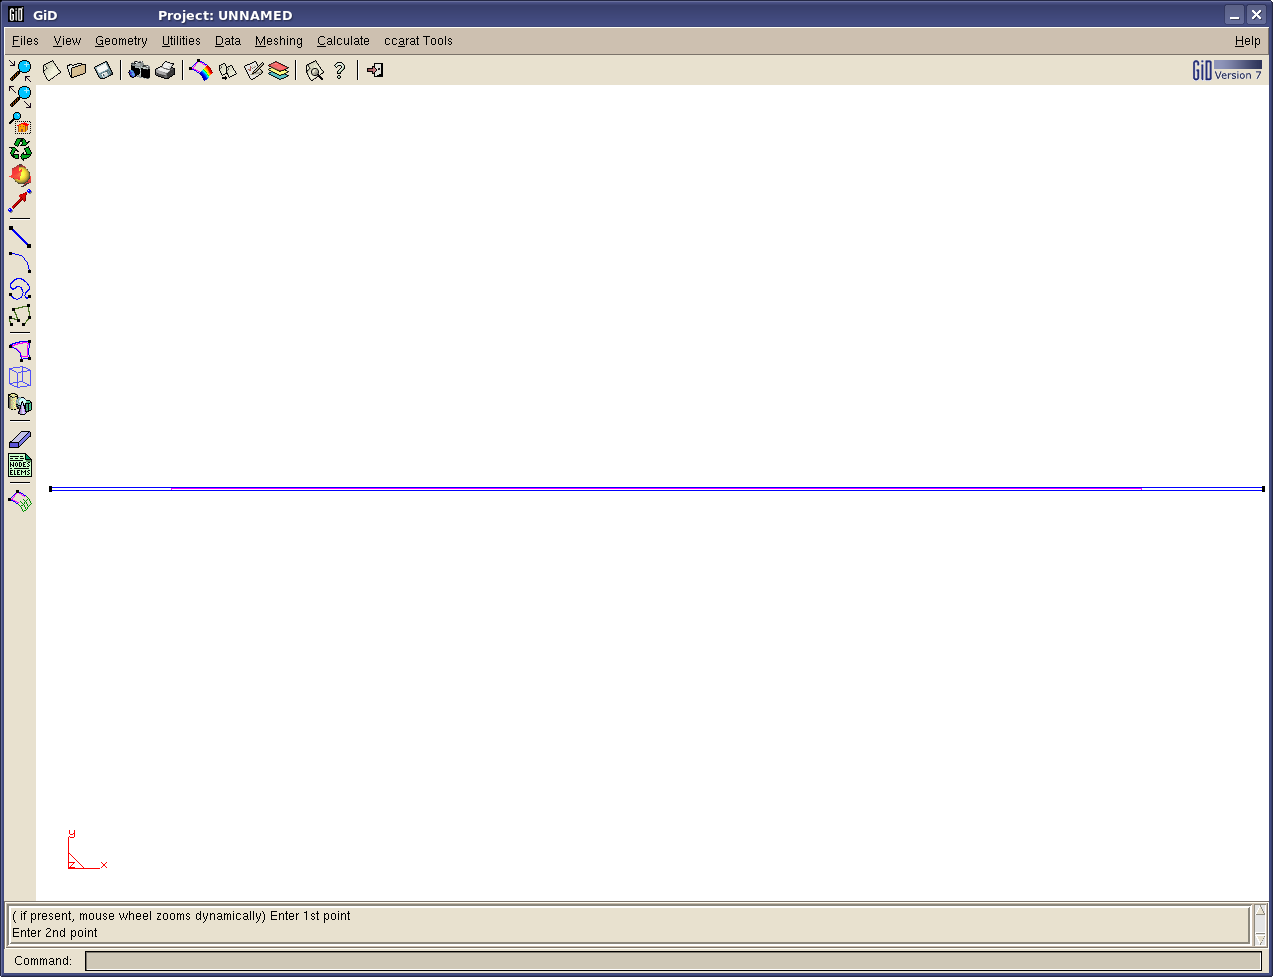
\includegraphics[width=1\columnwidth,keepaspectratio]{Bilder/structure_01}


\caption{\label{tut_fsi:3.1} The bottom of the chamber in GID}
\end{figure}


For a structural problem you only need one layer, so don't worry about
it and simply draw the geometry you need as we did here. To tell GID
that you have your material between this closed bunch of lines, you
have to specify a surface or volume (in 3D, displayed light green)
in between (which then can be linked to a material). Surfaces can
only be generated between lines or splines and Volumes only between
surfaces. In order to make meshing easier, always try to use very
simple surfaces and volumes (e.g. rectangles). Try to split your geometry
into several easy parts.


\subsection{Material and finite elements}

\begin{itemize}
\item Choose \emph{Data$\to$Materials$\to$Structure} and check if \emph{StVernantKirc}
is selected. Change the

\begin{itemize}
\item \emph{young modulus} to \emph{250}, 
\item \emph{Poisson's ratio} to \emph{0.3, }
\item \emph{density} to \emph{500} and 
\item \emph{Assign} the surface (click on \emph{Assign$\to$Surfaces} and
pick one of the light red edges) you created previously. 
\item Check this step in the materials menu via \emph{Draw$\to$This Structure}.
As you see, the assigned components are then highlighted in some color.
Go to \emph{finish} to leave and
\item \emph{Close} to return.
\end{itemize}
\end{itemize}
\emph{StVernantKirc} describes linear elastic material behaviour.
Here you can also, among others, choose e.g. plastic behaviour.

In more dimensional problems you have to deal with volumes, where
you then need the \emph{Assign-Volumes} button.

The \emph{Draw$\to$This Structure} button is very helpful if you
had troubles during the design and deleted some things. Here you can
check, if still everything is selected.

\begin{itemize}
\item As we want to choose the necessary finite element type next, we have
to enter the \emph{SingleLayer} menu via \emph{Data$\to$Conditions$\to$SingleLayer}.
On the top of this menu you can choose between \emph{points}, \emph{lines},
\emph{surfaces} and \emph{volumes}. Click the 

\begin{itemize}
\item \emph{surface} button, choose 
\item \emph{Wall} from the pulldown menu and 
\item \emph{Assign} our rectangle. 
\item You can check again with \emph{Draw$\to$Colors}.
\end{itemize}
\end{itemize}
In SingleLayer, in the element menu, you have the possibility to adjust
parameters of the element, like number of Gauss points, etc.

If you are dealing with a 3D problem, you have to click on the volumes
button and \emph{Assign} e.g. the \emph{Brick1} element.


\subsection{Numbering and boundary conditions}

BACI needs a numbering for all used design elements (points, lines,..),
which we have to generate manually.

All the next steps are done in \emph{SingleLayer}.

\begin{itemize}
\item To generate the numbering, choose e.g. 

\begin{itemize}
\item \emph{Point} and 
\item \emph{Design Node Number} from the pull down menu. 
\item \emph{Assign} all four points of our geometry.
\item Confirm with finish. 
\item Check with \emph{Draw$\to$Colors}. 
\end{itemize}
\item The same has to be done for all lines (choose \emph{Design Line Number})
and 
\item surfaces (\emph{Desingn Surface Number}).
\end{itemize}
The numbering is quite often a source of problems if you changed something
during the design. In order to avoid a complete renumbering, you can
take advantage of an automatic tool, which you can find via \emph{Utilities-Renumber}.
Additionally, you can also use \emph{Utilities-Repair} to make sure
the geometry is okay (no gaps, etc.).

Now you can focus on the boundary conditions: We want to lock the
displacements of the left and right vertical lines, as they connect
the flexible bottom with the rigid walls. 

\begin{itemize}
\item In SingleLaver click the \emph{}

\begin{itemize}
\item \emph{line} button and choose 
\item \emph{L Dirich} from the pull-down menu. 
\item Tick \emph{1} and \emph{2} (x- and y-direction) to \emph{On} and leave
the values below to \emph{0.0} as default.
\item Then \emph{Assign} the left and right line.
\end{itemize}
\end{itemize}
The weight of the fluid on the bottom has to be modeled next, so we
have to specify a Neumann boundary condition on the upper line of
the rectangle, with a constant value for the whole line. 

\begin{itemize}
\item In \emph{SingleLayer} click the 

\begin{itemize}
\item \emph{line} button and pick 
\item \emph{L Neum} from the pulldown menu.
\item Set the \emph{y}-direction (\emph{2}) to \emph{On}, the value to \emph{-1}
(the line weight of the fluid) and 
\item \emph{Assign} the uppermost line of our rectangle.
\end{itemize}
\end{itemize}
Generally, to lock displacements or to set them to a given value you
can choose between \emph{P-}, \emph{L-}, \emph{S-} or \emph{V Dirich}
(for points, lines, surfaces, and - yes - volumes). Values \emph{1},\emph{2}
and \emph{3} represent the displacements in x-, y- and z-direction.

In combination with a Neumann boundary condition, it is possible to
create a time and/or location dependent load. In \emph{SingleLayer}
you can specify a certain \emph{Load Funct} (function dependent on
a physical coordinate) or a \emph{Load Curve} (dependent on time)
for dynamic problems. All the ticked functions, curves and the value
are multiplied to a resultant loading. The functions or curves can
be specified via \emph{Data$\to$Problem Data$\to$Functions} or to
\emph{Data$\to$Interval Data}.


\subsection{Meshing}

The most controllable way to do the meshing is by dividing lines of
our surface into several elements and then to mesh these divided lines
(like in other commercial FE-software).

\begin{itemize}
\item Close SingleLayer and go to \emph{Meshing$\to$Structured$\to$Surfaces}.
You are then asked for a surface. 

\begin{itemize}
\item Click on an edge of our rectangular surface and hit 
\item \emph{esc}.
\item In the following window you are asked for the divisions to be made,
where you type in \emph{1} (one element in vertical direction is enough
as the bottom is only 0.002 thick) and click 
\item \emph{ok}. 
\item Pick one of our vertical lines (the other one is selected automatically)
and hit 
\item \emph{esc}.
\item Now we have to repeat this step for the horizontal line. Type in \emph{64}
and click 
\item ok. Then 
\item select one of the horizontal lines and hit 
\item \emph{esc} twice. 
\end{itemize}
\item Go to \emph{Meshing$\to$Generate}. Ignore the value window (it is
necessary for unstructured meshing). At this point you should see
the meshed, green structure right in front of you, see \ref{tut_fsi:3.2}.
\end{itemize}
%
\begin{figure}[h]
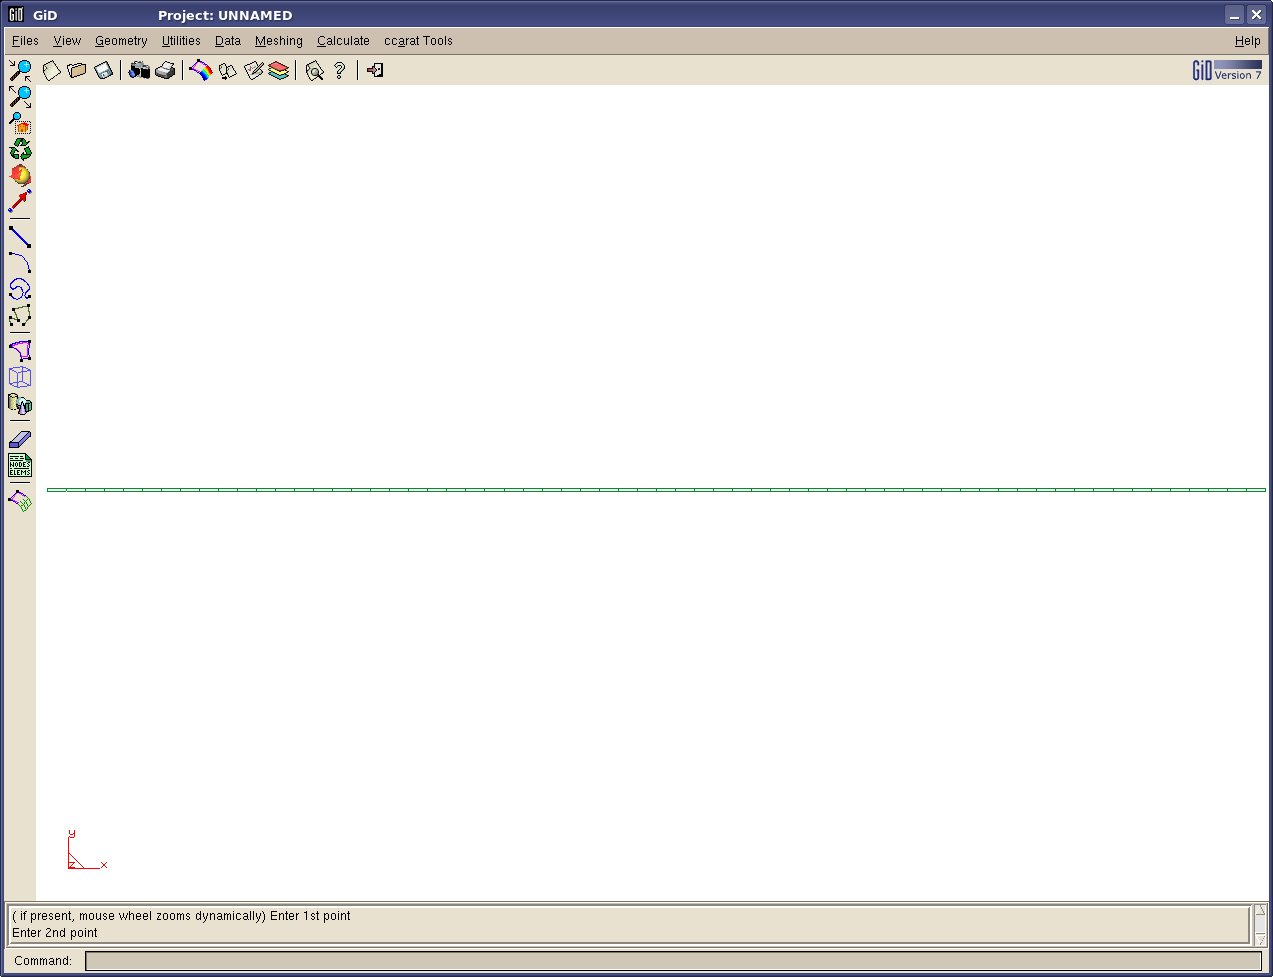
\includegraphics[width=1\columnwidth]{Bilder/structure_02}


\caption{\label{tut_fsi:3.2} Mesh of the bottom}
\end{figure}


If you want to mesh something in 3D, just go to \emph{Meshing$\to$Structured$\to$Volumes}
and do the same like in 2D. Usually you get problems if you have complicates
geometries, so try to keep them as simple as possible.

You can shift between the mesh view and the geometry view by means
of the \emph{Toggle geometry$\to$mesh view} button in the left tool
bar.

Always make sure to regenerate the mesh if you changed something in
the geometry or in \emph{SingleLayer}, even if you did the renumbering.


\subsection{Solving}

\begin{itemize}
\item If you didn't save your example yet, do so to give GID a directory
for the next step. 
\item To write the text input file for BACI, simply click \emph{Calculate$\to$Calculate}.
This will write the \emph{{*}.dat} file in the directory of your example.
\item To start the solver use the call \emph{./cca\_fc6\_ser.fast ../your\_example.dat
../resultdirectory/result\_prefix} (in the CCARAT directory). The
results (\emph{{*}.flavia.res} and some others) are then written to
the result directory with the prefix you chose.
\end{itemize}

\subsection{Postprocess}

\begin{itemize}
\item To do the postprocessing shift GID via \emph{Files$\to$Postprocess}.
Then 
\item open the \emph{{*}.flavia.res} of your example and 
\item plot the results via \emph{View results$\to$...}, see also \ref{tut_fsi:3.3}.
\end{itemize}
%
\begin{figure}[h]
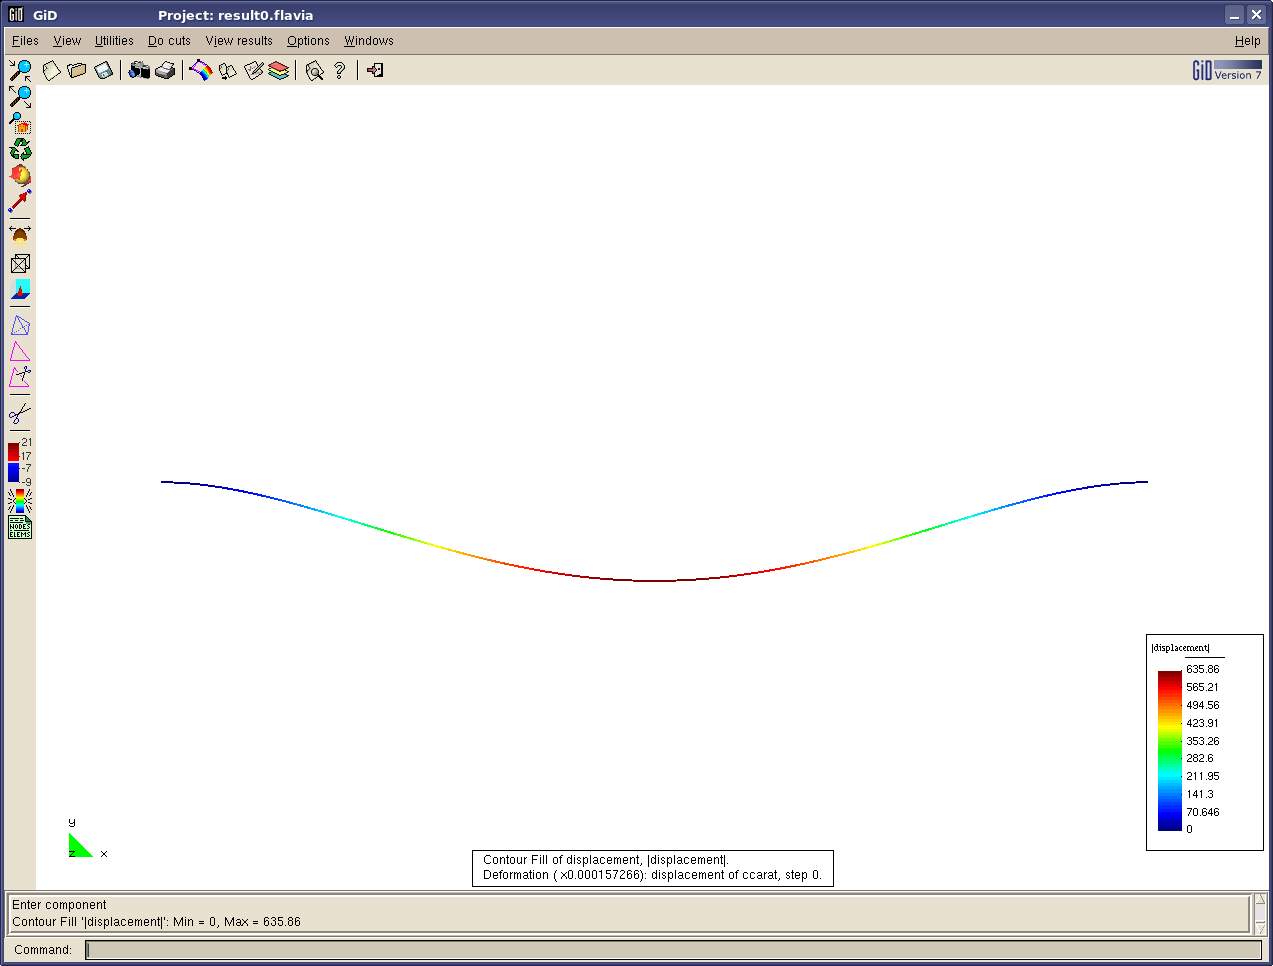
\includegraphics[width=1\columnwidth]{Bilder/structure_03}


\caption{\label{tut_fsi:3.3} Displacement of the bottom}
\end{figure}


All lessons learned here are necessary for the next chapter and won't
be explained again, so keep them in mind.


\section{The fluid try}

Here we are going to simulate the driven cavity with a rigid bottom,
but everything else as we want to have it in the final FSI example.


\subsection{General}

\begin{itemize}
\item Activate \emph{Data$\to$Problem Type$\to$lnm\_general} as basis.
\item In \emph{Data$\to$Problem Data$\to$General Problem Data} check if 

\begin{itemize}
\item \emph{Problem Typ} is set to \emph{Fluid}, 
\item \emph{Number of Fields} is set to \emph{one,} 
\item \emph{Max NumDOF} is set to \emph{four} and 
\item \emph{Static/Dynamic} is set to \emph{Dynamic.}
\end{itemize}
\end{itemize}
We choose four degrees of freedom, although we have a two dimensiona
problem and three would be sufficient (two velocities and the pressure).
Well, you can type in three, but basically it doesn't matter. 

Here \emph{Dynamic} has to be selected, as we have a time dependent
velocity. But even in a stationary fluid problem you have to set it
to \emph{Dynamic} as in fluid simulations you always have to start
the velocities from zero with a time-dependent curve. to get good
solutions.


\subsection{Geometry}

As we later have to define the Dirichlet boundary condition at the
inlet, it has to be a separate line. So the easiest way to specify
our fluid is to use two rectangles (lets say the upper rectangle and
a u-profile for the lower one, so you don't have two lines laying
on each other where they meet).

\begin{itemize}
\item Use the corners \emph{0,0} and \emph{1,1} for the lower and \emph{0,1}
and \emph{1,1.1} for the upper rectangle.
\item Generate two surfaces in between the lines. 
\end{itemize}
What you have now should look like \ref{tut_fsi:4.1}.

%
\begin{figure}[h]
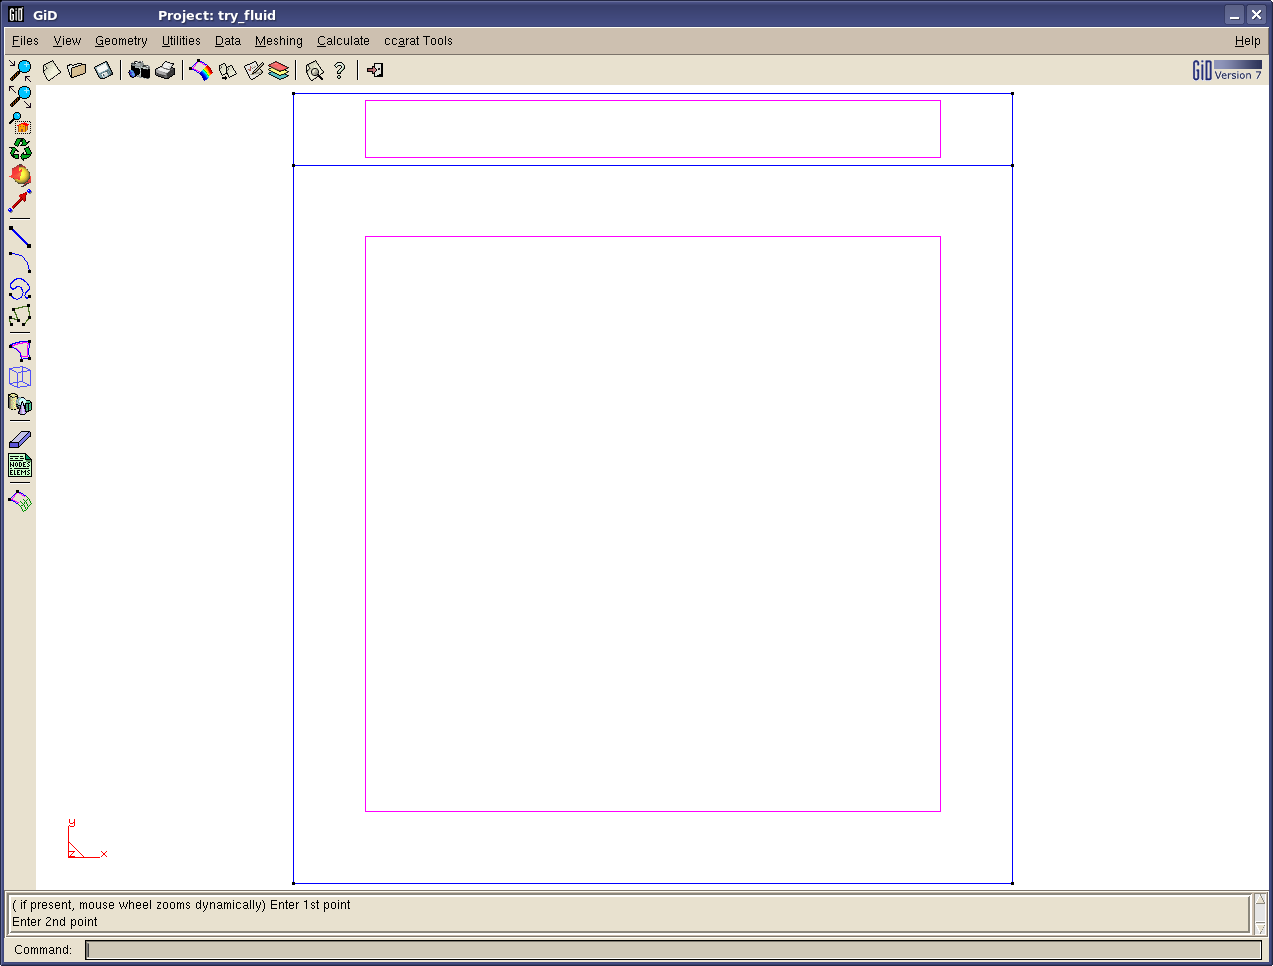
\includegraphics[scale=0.4]{Bilder/fluid_01}


\caption{\label{tut_fsi:4.1} The fluid in the chamber}
\end{figure}



\subsection{Material and finite element}

\begin{itemize}
\item Go to \emph{Data$\to$Materials$\to$Fluid} and adjust the fluid parameters
to 

\begin{itemize}
\item \emph{density = 1, }
\item \emph{viscosity = 0.01}. Then 
\item \emph{Assign} our two rectangles. 
\end{itemize}
\item For the specification of the element, go to 

\begin{itemize}
\item \emph{SingleLayer} and click the 
\item \emph{Surfaces} button. Choose the 
\item \emph{Fluid2} element from the pull-down menu and 
\item \emph{Assign} our two rectangular surfaces, as they make up our fluid.
\end{itemize}
\item In order to prevent oscillations in the solution, we have to stabilize
the fluid. Click the 

\begin{itemize}
\item \emph{surface} button in \emph{SingleLayer,} choose the 
\item \emph{Fluid Surface Stab} from the pulldown menu and
\item \emph{Assign} our two rectangles.
\end{itemize}
\end{itemize}
In the \emph{Fluid2} menu make sure that \emph{Net Algo} is set to
\emph{Euler}, the default algorithm. We are going to use the \emph{ALE}
algorithm later in the FSI section.

The stabilisation has to be made seperately here, which is a little
clumsy but necessary for science. Just don't forget about it.


\subsection{Numbering and boundary conditions}

\begin{itemize}
\item In \emph{Data$\to$Conditions$\to$SingleLayer} do the numbering as
you already know it from section 3.4. Here it is not much more complicated
than before, as we have six points, seven lines and two surfaces.
\end{itemize}
Again, the tricky part are the boundary conditions. \emph{SingleLayer}
is the one and only menu we need for the following:

\begin{itemize}
\item First we want to set the b.c.'s at the walls, so click the

\begin{itemize}
\item line button. Activate 
\item \emph{1} and \emph{2} (velocity in x- and y-direction) and leave them
at default values (\emph{0.0}, because we have no slip at the wall).
\item Assign the according lines (the two lower vertical- and the bottom-line
of the container). 
\end{itemize}
\item Don't forget the points! All four lower points need to be treated
like above, too.
\item For the intake we have to concentrate a bit more: In \emph{SingleLayer}
click the

\begin{itemize}
\item \emph{lines} button and choose 
\item \emph{L Dirich}. Our triangle-shaped, time dependent velocity field
will point towards the x-direction so we switch 
\item \emph{1} to \emph{on} and set the value to \emph{1}. Further we want
a \emph{load curve} to be multiplied to this constant factor, to give
it a time dependency, so we switch 
\item \emph{Load Curve value 1} to \emph{1}. To make the field also dependent
of the y-coordinate, we have to switch 
\item \emph{Load Funct value 1} to \emph{1}. 
\item Now \emph{Assign} the intake line.
\end{itemize}
\item Next we are going to define the expressions for \emph{curve 1} and
\emph{funct 1}. Go to 

\begin{itemize}
\item \emph{Data$\to$Interval Data} and pick
\item \emph{curve 1}. Switch it to 
\item \emph{on} and choose 
\item \emph{EXPR} from the pulldown menu. We type in 
\item \emph{1-cos(2{*}t{*}pi/5)}. Go to 
\item \emph{Accept data} and 
\item \emph{Close}. Quite the same has to be done for the load function,
so we go to 
\item \emph{Data$\to$Problem Data$\to$Functions}. Switch 
\item \emph{Funct 1} to 
\item \emph{on} and activate 
\item \emph{EXPR}. As BACI uses absolute coordinates for functions, we have
to use 
\item \emph{10{*}(y-1)} to give it the triangular shape as our line is between
0,1 and 0,1.1. 
\end{itemize}
\end{itemize}
The velocity field now results from a multiplication of curve 1, function
1 and the maximum value (here: 1).

So far for the intake.

\begin{itemize}
\item Use the uppermost horizontal line for b.c. 

\begin{itemize}
\item x-velocity = \emph{1} and, as it has the same time dependency like
the intake, pick also 
\item \emph{curve 1} as factor.
\end{itemize}
\end{itemize}
The exhaust doesn't need a boundary condition (we just want the pressure
to be zero there) so we can skip it in this section. 


\subsection{Meshing}

\begin{itemize}
\item Use the same procedure like in the structural example. Mesh our example
with 

\begin{itemize}
\item 64x7 and 
\item 64x64 elements, respectively. This should be a good compromise for
the result we need.
\end{itemize}
\item Go to \emph{Calculate$\to$Calculate} to write the input file.
\end{itemize}

\subsection{Solving}

\begin{itemize}
\item To start the solver use the same command in the console like for the
structural example.
\end{itemize}

\subsection{Postprocess}

For the postprocess you have to use another softare called \emph{paraview}. 

\begin{itemize}
\item Before you can open our results there, you have to filter them with
the call (inside the ccarat directory): \emph{post\_drt\_ensight --file=result\_prefix}
\item After this open \emph{paraview}, go to 

\begin{itemize}
\item \emph{File$\to$Open Data} and select the filtered \emph{{*}.case
file}. 
\item Select the time step in the \emph{Select Time Value} window on the
left and 
\item shift \emph{Byte order} to \emph{little endian}. Go to 
\item \emph{Accept} to activate the display.
\item In the \emph{Display tab} (section \emph{Color}) you can choose now
between \emph{Point pressure} and \emph{Point velocity}, whatever
you want to display.
\item For the scale, activate the \emph{Scalar bar} button in the \emph{View
section}. 
\end{itemize}
\end{itemize}
See also \ref{tut_fsi:4.2} for comparison.

%
\begin{figure}[h]
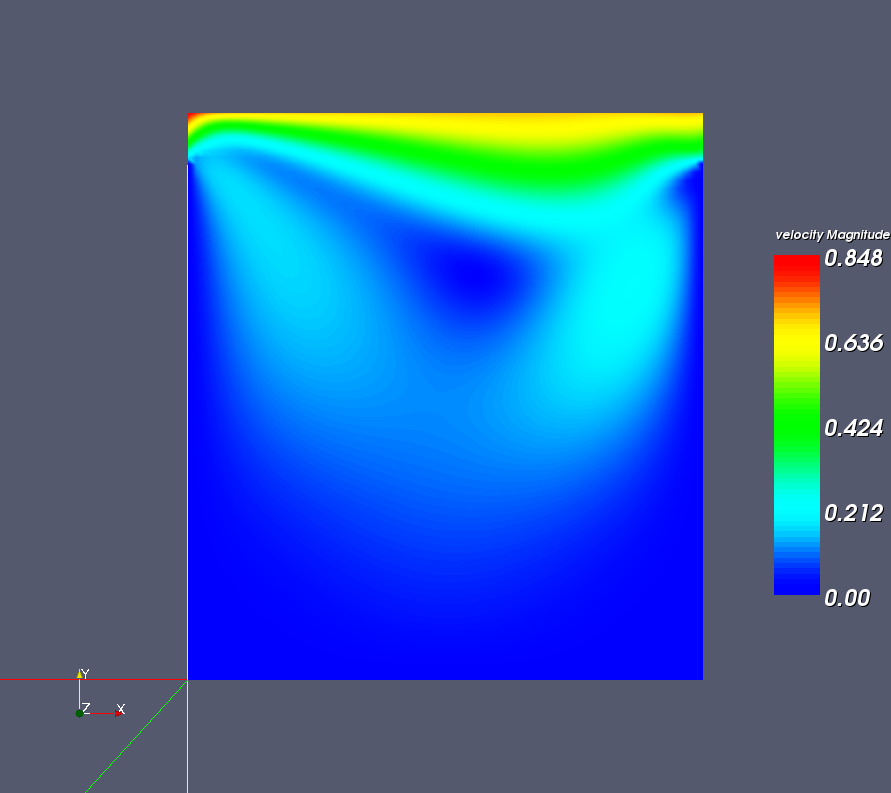
\includegraphics[scale=0.4]{Bilder/fluid_02}


\caption{\label{tut_fsi:4.2} Velocity distribution at timestep 200}
\end{figure}



\section{Finally, the FSI example}


\subsection{General}

\begin{itemize}
\item Set \emph{lnm\_general} as basis and set \emph{}
\item \emph{Data-Problem Data$\to$General Problem Data}. Here we have 

\begin{itemize}
\item three fields (structure, fluid and ALE), 
\item four degrees of freedom and a 
\item dynamic problem (like when we dealt with the simple fluid problem). 
\item Problem Typ is Fluid Structure Interaction now.
\end{itemize}
\end{itemize}
The FSI problem, in comparison to the previous ones, needs some certain
definitions due to the coupling between structure mesh and fluid mesh.

\begin{enumerate}
\item An ALE mesh, which is automatically generated in the fluid, and needs
some certain boundary conditions. The ALE is responsible for the movement
of the fluid mesh, so that the coupling elements of the fluid move
like the deformed structure.
\item Two different layers where structure and the fluid are specified.
\item Coupling lines which are moved and deteriorated due to the deformation
of the structure and make sure, that there is no gap between structure
and fluid.
\end{enumerate}

\subsection{Geometry}

\begin{itemize}
\item We need to generate two layers first. Click the 

\begin{itemize}
\item \emph{Layers} button in the upper tool bar and type in the name 
\item \emph{Structure} in the command line of the layers tab. Then click 
\item \emph{New} and in the upper part of the tab the \emph{Structure} layer
should be displayed. The next thing we do here is to rename \emph{Layer0}. 
\item Mark it in the upper list of the tab, type 
\item \emph{Fluid} into the command line and click 
\item \emph{Rename}.
\end{itemize}
\end{itemize}
The layers menu should look like in \ref{tut_fsi:5.1} now.

%
\begin{figure}[h]
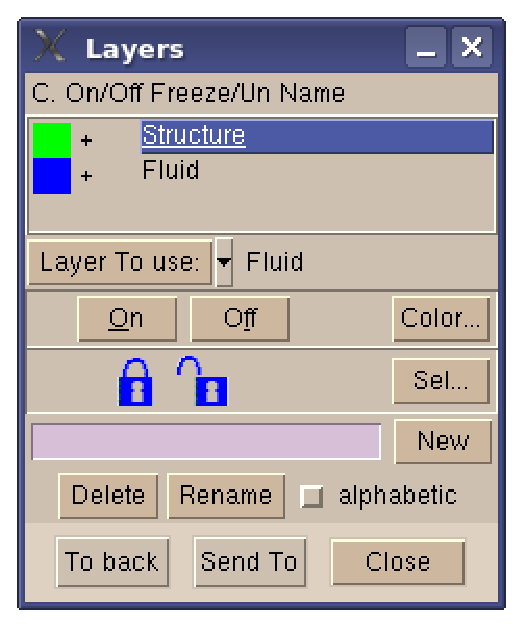
\includegraphics[scale=0.6]{Bilder/fsi_01}


\caption{\label{tut_fsi:5.1} Layers necessary}
\end{figure}


\begin{itemize}
\item Now we want to draw our bottom, so mark the \emph{}

\begin{itemize}
\item \emph{Structure} layer and click
\item \emph{On}. Do the same, but with \emph{}
\item \emph{Off} for \emph{Fluid} to deactivate the other one. 
\item Now draw a rectangle (like in 3.2) with corners \emph{0,0} and \emph{1,-0.002}. 
\item Generate a surface in between.
\end{itemize}
\item Now we move on to the fluid. Activate the \emph{}

\begin{itemize}
\item \emph{fluid} layer and turn 
\item \emph{Off} the structure layer to prevent complications. You should
have an {}``empty'' workspace again. 
\item Create the two rectangular surfaces like in 4.2.
\end{itemize}
\item Now activate the \emph{structure} layer again and check if you have
the geometry like in \ref{tut_fsi:5.2}.
\end{itemize}
%
\begin{figure}[h]
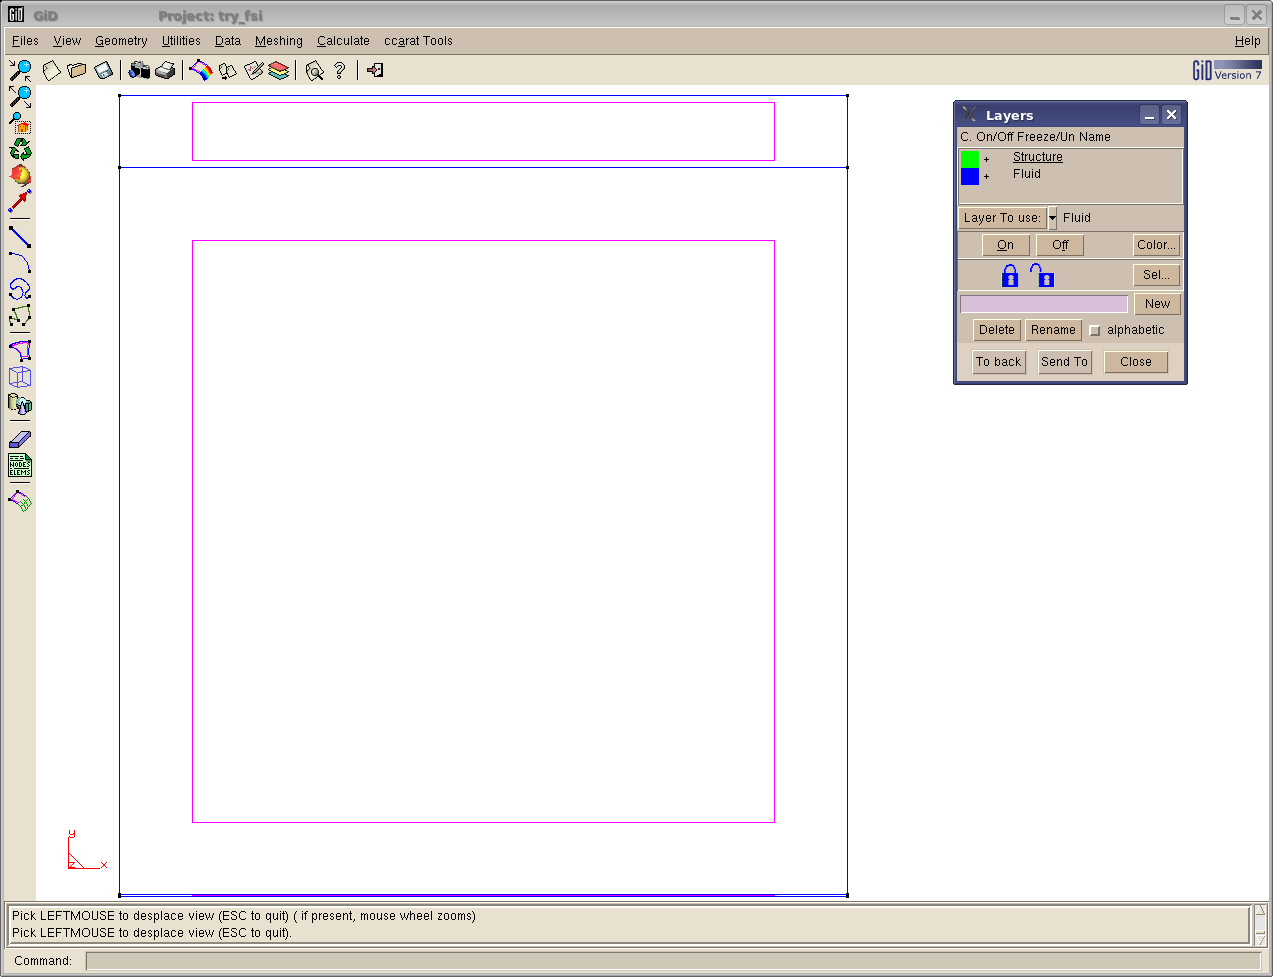
\includegraphics[scale=0.4]{Bilder/fsi_02}


\caption{\label{tut_fsi:5.2} FSI geometry and layers}
\end{figure}


The easiest way to make sure about the lines laying on each other
right from the beginning is to draw them by coordinates. Experienced
users can also try to copy the according design elements from one
layer to the other via the \emph{Copy/Transform} button in the upper
tool bar. 


\subsection{Material and finite element}

\begin{itemize}
\item Activate the \emph{structure} layer only. Go to \emph{Data$\to$Materials}
and 

\begin{itemize}
\item assign the bottom as structure with material parameters like in 3.3. 
\item In \emph{SingleLayer} specify the finite element you need for the
structure (\emph{Wall} element with default settings).
\end{itemize}
\item Now activate the \emph{fluid} layer only. Go to 

\begin{itemize}
\item \emph{Data$\to$Materials-Fluid}, set 
\item \emph{density} and 
\item \emph{viscosity} as in 4.3 and 
\item \emph{Assign} the two rectangles. Move on to 
\item \emph{SingleLayer}. The according finite element for us is the 
\item \emph{Fluid2} element. Use it for the two surfaces, but make sure
to set 
\item \emph{Net Algo} to \emph{ALE} and activate the 
\item \emph{Create Ale} button before you 
\item \emph{Assign}. 
\item Use the \emph{Fluid Surface Stab} for the two rectangles, like in
4.3.
\end{itemize}
\item Before we move to the boundary conditions, we have to activate the
material parameters for the ALE first (some default values, which
are needed by the solver). Go to

\begin{itemize}
\item \emph{Data$\to$Materials$\to$Structure} and set for 
\item \emph{MAT Struct StVenantKir} some default parameters (e.g. \emph{1},
\emph{0.3}, \emph{1}) and then click 
\item \emph{Close}. You are then asked if you want to save the changed parameters,
which you confirm with \emph{}
\item \emph{Yes}.
\end{itemize}
\end{itemize}
The \emph{Create ALE} button (when you define the fluid element) is
necessary, because the ALE is another mesh, which has to be generated
seperately. It also needs special boundary conditions, as we will
see later on.

This should also explain, why we have to set the \emph{NetAlgo} to
\emph{ALE}.


\subsection{Numbering and boundary conditions}

\begin{itemize}
\item The numbering is the same procedure like in 3.4 and 4.4. The only
thing worth mentioning here is that it is easier to do this process
layer by layer. So switch on the \emph{structure} layer only, number
its elements and then do the same for the \emph{fluid} layer.
\end{itemize}
Generally here you have to specify all b.c.'s for structure and fluid
and some additional ones for the ALE.

\begin{itemize}
\item Activate the structure layer only. 

\begin{itemize}
\item Use the left and right vertical lines for Dirichlet b.c. with displacement
set to 
\item \emph{0} and \emph{0}. 
\item Use all four points and set their displacement also to \emph{0} and
\emph{0}.
\item The uppermost line is our coupling element between the fluid and the
structure, so we specify it as \emph{FSI Coupling Line} (you find
it in \emph{SingleLayer}) with \emph{Field structure}.
\end{itemize}
\end{itemize}
So far for the bottom.

\begin{itemize}
\item Now we activate the fluid layer only. 

\begin{itemize}
\item Use the four lower points and 
\item the two lower vertical lines for Dirichlet b.c. with 
\item \emph{0} and \emph{0} velocity.
\item The upper left vertical line (the inlet) again has the triangle shaped
velocity distribution. To specify it, use the same procedure as in
4.4.
\item The same has to be done for the uppermost line (time dependency!),
see also 4.4.
\item Pick the lowest horizontal line and assign it as \emph{FSI Coupling
Line} with \emph{Field fluid}.
\end{itemize}
\item The last thing for us to do before meshing is to work on the ALE:
We have to tell the code, which part of the fluids mesh which will
remain stationary. Here these are 

\begin{itemize}
\item all points and 
\item all the outer lines except of the bottom line. 
\item \emph{Assign} them as \emph{P AleDirich} or \emph{L AleDirich} (also
in \emph{SingleLayer}), respectively with displacement \emph{0} and
\emph{0}. 
\end{itemize}
\end{itemize}
Make sure to only use geometry of the fluid layer for fluid b.c.'s
and only geometry from the structure layer for structure b.c.'s. The
easiest way to accomplish this is by switching the one not needed
to \emph{Off} during the selection, as we did right from the beginning. 

The coupling elements are geometries, which make sure, that the fluid
and the structure deteriorate in the same way. They serve two purposes:

\begin{enumerate}
\item They ensure, that fluid and structure deform equally there and
\item that the fluid has also the same tangential velovity as the structure
(no slip at the surface). 
\end{enumerate}

\subsection{Meshing}

\begin{itemize}
\item Meshing is the same procedure like in 3.5 and 4.5, except of it, that
you should mesh structure and fluid seperately, with the according
layer activated only. This makes picking of the lines easier and produces
less problems. Mesh the surfaces of our example with 

\begin{itemize}
\item 64x7, 
\item 64x64 and 
\item 64x1 elements, respectively.
\end{itemize}
\end{itemize}
Keep in mind, that structure and fluid have to have congruent meshes
at the coupling elements. 


\subsection{Solving}

\begin{itemize}
\item Go to Calculate\emph{$\to$}Calculate to write the \emph{{*}.dat}
file. 
\item Again, use the call \emph{./cca\_fc6\_ser.fast ../file\_directory/example.dat
../file\_direc-tory/result\_prefix} to start the solver and
\item \emph{./post\_drt\_ensight --file=result} to filter the results for
postprocess.
\end{itemize}
If you get convergence problems during the run, it might help to shift
to another solver. Terminate the run and change the \emph{{*}.dat}
file to do this. In the header of the dat file (\emph{General Data
File CCARAT}) you find the section \emph{FLUID SOLVER}, \emph{STRUCT
SOLVER} and \emph{ALE SOLVER}. Change all the first (and possibly
second) lines, where \emph{SOLVER} is written, from \emph{Aztec} to
\emph{UMFPACK}, save and rerun.


\subsection{Postprocess}

\begin{itemize}
\item Use \emph{paraview} to evaluate the example. There you have the option
to display pressure-, velocity- or displacement distribution (here:
displacement of the ALE, so interesting for us are only the values
at the coupling line). For comparison see also \ref{tut_fsi:5.3} and
\ref{tut_fsi:5.4}.
\end{itemize}
%
\begin{figure}[h]
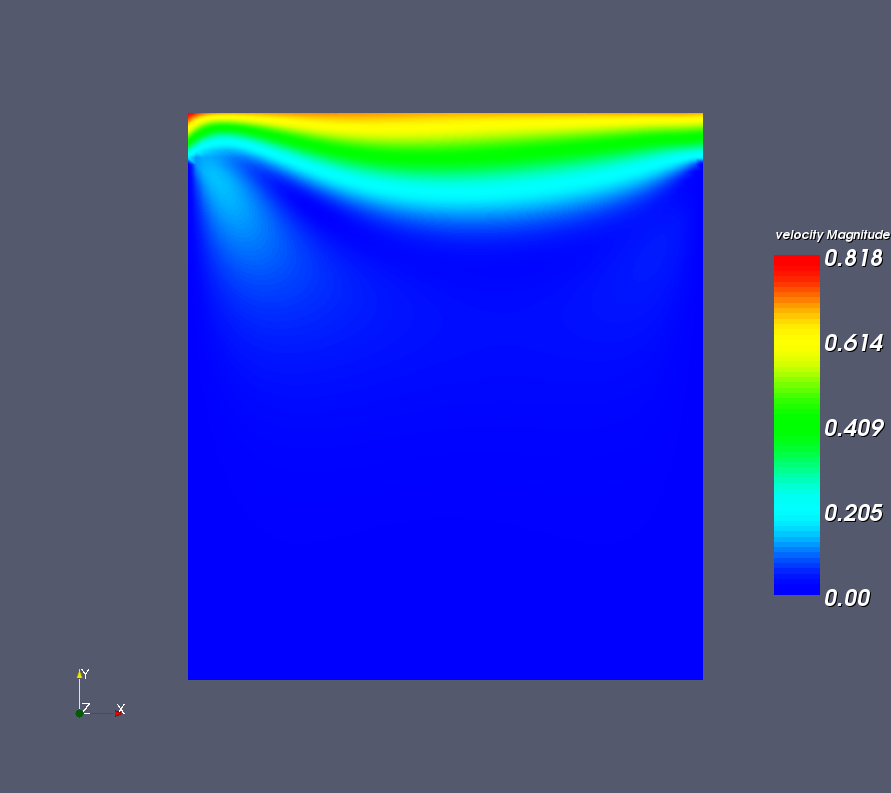
\includegraphics[scale=0.4]{Bilder/fsi_03}


\caption{\label{tut_fsi:5.3} Velocity distribution at timestep 35}
\end{figure}


%
\begin{figure}[h]
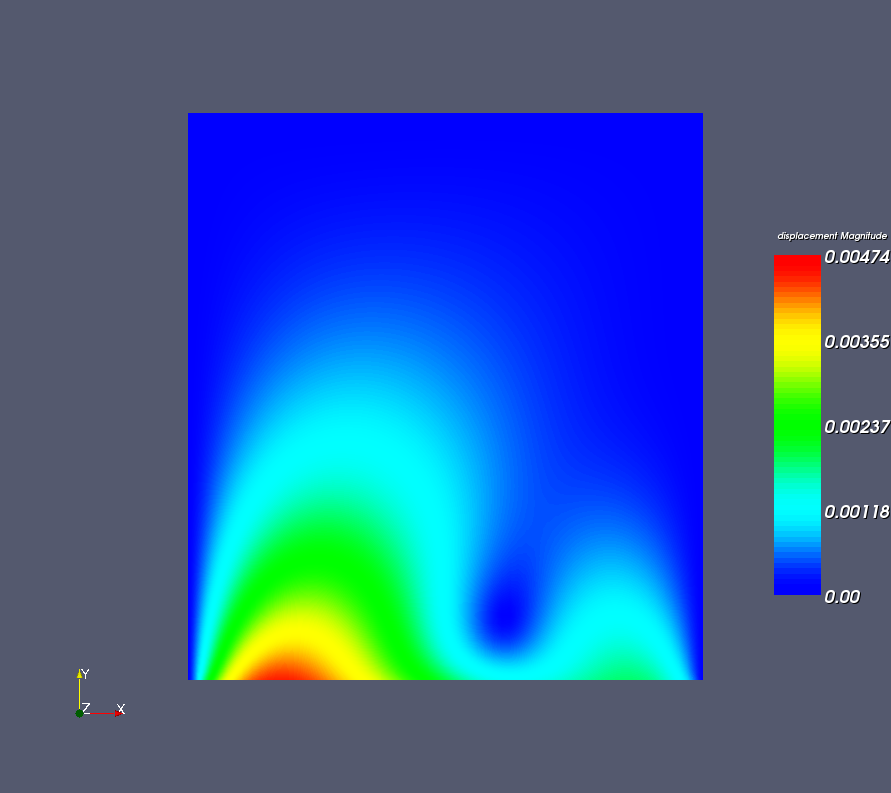
\includegraphics[scale=0.4]{Bilder/fsi_04}


\caption{\label{tut_fsi:5.4} Displacement distribution at timestep 35}
\end{figure}
